%\documentclass[fleqn,14pt,a4paper,twoside]{extarticle}
\documentclass[a4paper, 11pt]{extarticle}
%%% Работа с русским языком
\usepackage{cmap}					% поиск в PDF
\usepackage{mathtext} 				% русские буквы в формулах
\usepackage[T2A]{fontenc}			% кодировка
\usepackage[utf8]{inputenc}			% кодировка исходного текста
\usepackage[english,russian]{babel}	% локализация и переносы
%\usepackage[tmargin=4cm,bmargin=4cm,lmargin=2cm,rmargin=2cm,asymmetric,headheight=50pt,bindingoffset=1cm]{geometry}
\usepackage[tmargin=1.5cm,bmargin=1.5cm,lmargin=2cm,rmargin=1.5cm,headheight=50pt]{geometry}
\usepackage{comment} % enables the use of multi-line comments (\ifx \fi) 
\usepackage{lipsum} %This package just generates Lorem Ipsum filler text. 
\usepackage{fullpage} % changes the margin
%\usepackage[a4paper, total={7in, 10in}]{geometry}
\usepackage[fleqn]{amsmath}
\usepackage{amssymb,amsthm}  % assumes amsmath package installed
\newtheorem{theorem}{Theorem}
\newtheorem{corollary}{Corollary}
\usepackage{graphicx}
\usepackage{tikz}
\usetikzlibrary{arrows}
\usepackage{verbatim}
\usepackage[numbered]{mcode}
\usepackage{float}
\usepackage{tikz}
    \usetikzlibrary{shapes,arrows}
    \usetikzlibrary{arrows,calc,positioning}

    \tikzset{
        block/.style = {draw, rectangle,
            minimum height=1cm,
            minimum width=1.5cm},
        input/.style = {coordinate,node distance=1cm},
        output/.style = {coordinate,node distance=4cm},
        arrow/.style={draw, -latex,node distance=2cm},
        pinstyle/.style = {pin edge={latex-, black,node distance=2cm}},
        sum/.style = {draw, circle, node distance=1cm},
    }
\usepackage{xcolor}
\usepackage{mdframed}
\usepackage[shortlabels]{enumitem}
%\usepackage{indentfirst}
\usepackage{hyperref}

\hypersetup{
    colorlinks=true,
    linkcolor=blue,
    filecolor=magenta,      
    urlcolor=cyan,
}
\renewcommand{\thesubsection}{\thesection.\alph{subsection}}

\newenvironment{problem}[2][Problem]
    { \begin{mdframed}[backgroundcolor=gray!20] \textbf{#1 #2} \\}
    {  \end{mdframed}}

% Define solution environment
\newenvironment{solution}
    {\textit{Solution:}}
    {}

\renewcommand{\qed}{\quad\qedsymbol}


\usepackage{fancyhdr}
\usepackage{emptypage}
\fancyhead{}
\fancyfoot{}
\fancyhead[LE,RO]{
\includegraphics [width=.3\textwidth] {logo.png}}
\fancyfoot[LE,RO]{\thepage}
\pagestyle{fancy}
\graphicspath{{../../tex_templates/figures/}}

% code listing settings
\usepackage{listings}
\lstset{
    language=Python,
    basicstyle=\ttfamily\small,
    aboveskip={1.0\baselineskip},
    belowskip={1.0\baselineskip},
    columns=fixed,
    extendedchars=true,
    breaklines=true,
    tabsize=4,
    prebreak=\raisebox{0ex}[0ex][0ex]{\ensuremath{\hookleftarrow}},
    frame=lines,
    showtabs=false,
    showspaces=false,
    showstringspaces=false,
    keywordstyle=\color[rgb]{0.627,0.126,0.941},
    commentstyle=\color[rgb]{0.133,0.545,0.133},
    stringstyle=\color[rgb]{01,0,0},
    numbers=left,
    numberstyle=\small,
    stepnumber=1,
    numbersep=10pt,
    captionpos=t,
    escapeinside={\%*}{*)}
}



%%%%%%%%%%%%%%%%%%%%%%%%%%%%%%%%%%%%%%%%%%%%%%%%%%%%%%%%%%%%%%%%%%%%%%%%%%%%%%%%%%%%%%%%%%%%%%%%%%%%%%%%%%%%%%%%%%%%%%%%%%%%%%%%%%%%%%%%
\begin{document}
%Header-Make sure you update this information!!!!
%\noindent
%%%%%%%%%%%%%%%%%%%%%%%%%%%%%%%%%%%%%%%%%%%%%%%%%%%%%%%%%%%%

\noindent \LARGE{\textbf{Course: WebDev -- Django Start.}} \hfill  \\ 
%\vspace{0.25em}
\textbf{Homework - 1. Solve}  \hfill  \\
%Email: veralevel@gethu.edu \hfill ID: 123456789 \\

\noindent Theme: Install instruments for work and basic HTML\hfill  \\
Level: beginner\\
Instructor: Mikhail Nakonechnyi \\
Due Date: $15^{th}$ February, 2020 \\
\noindent\rule{6.257in}{2.8pt}
%%%%%%%%%%%%%%%%%%%%%%%%%%%%%%%%%%%%%%%%%%%%%%%%%%%%%%%%%%%%

\begin{problem}{1}
Скачать \href{https://www.sublimetext.com/3}{Sublime Text 3} и установить. Все пункты выбирать по умолчанию.
\end{problem}

\noindent\rule{6.257in}{2.8pt}


%%%%%%%%%%%%%%%%%%%%%%%%%%%%%%%%%%%%%%%%%%%%%%%%%%%%%%%%%%%%

\begin{problem}{2}
Скачать \href{https://www.jetbrains.com/pycharm/download/#section=windows}{PyCharm Community} и установить. Все пункты выбирать по умолчанию.
\end{problem}

\noindent\rule{6.257in}{2.8pt}


%%%%%%%%%%%%%%%%%%%%%%%%%%%%%%%%%%%%%%%%%%%%%%%%%%%%%%%%%%%%%%%%%%%%%%%%%%%
% Problem 3
%%%%%%%%%%%%%%%%%%%%%%%%%%%%%%%%%%%%%%%%%%%%%%%%%%%%%%%%%%%%%%%%%%%%%%%%%%%
\begin{problem}{3}
Установка \href{https://git-scm.com/downloads}{Git Bash}. Все пункты выбирать по умолчанию.
\end{problem}

\noindent\rule{6.257in}{2.8pt}



%%%%%%%%%%%%%%%%%%%%%%%%%%%%%%%%%%%%%%%%%%%%%%%%%%%%%%%%%%%%

\begin{problem}{4}
Создать папку проекта \textbf{DjangoStart} у себя на ПК (для удобства лучше в папке \textbf{Документы/Documents} - код ниже, будет основан на этом расположении папки), далее скопировать в папку созданный репозиторий на \href{https://github.com/}{GitHub}. И проверить командой \textit{ls}, что папка репозитория скопировалась.\\
\textit{\textbf{Примечание: }} для тех, кто не создал на занятии -- репозиторий создается пустой с названием \textbf{django}. 
\begin{lstlisting}
cd ~/Documents/
mkdir DjangoStart
cd DjangoStart
git init
mkdir lesson1
cd lesson1
touch index.html
git add index.html
git config --global user.name "Your nickname"
git config --global user.email "name@mail.com"
git commit -m "initial commit"
git remote add origin https://github.com/$account$/$Repository name$.git
\end{lstlisting}
\end{problem}
\begin{solution}
%\begin{lstlisting}[label={list:second},caption=Sample Bash code.]
\begin{lstlisting}
cd ~/Documents/
mkdir DjangoStart
cd DjangoStart
git init
git clone https://github.com/$account$/$Repository name$.git
git config --global user.name "Your nickname"
git config --global user.email "name@mail.com"
\end{lstlisting}
\end{solution} 
\noindent\rule{6.257in}{2.8pt}


%%%%%%%%%%%%%%%%%%%%%%%%%%%%%%%%%%%%%%%%%%%%%%%%%%%%%%%%%%%%

\begin{problem}{5}
В папке \textbf{lesson1} нужно создать папку \textbf{homework} с помощью команд терминала \textbf{linux}. Далее скопировать файл \textbf{index.html} в эту папку.
\end{problem}
\begin{solution}
\begin{lstlisting}
cd ~/Documents/DjangoStart/lesson1/
mkdir homework
cp index.html homework/index.html
\end{lstlisting}
\end{solution} 
\noindent\rule{6.257in}{2.8pt}



%%%%%%%%%%%%%%%%%%%%%%%%%%%%%%%%%%%%%%%%%%%%%%%%%%%%%%%%%%%%%%%%%%%%%%%%%%%
% Problem 6
%%%%%%%%%%%%%%%%%%%%%%%%%%%%%%%%%%%%%%%%%%%%%%%%%%%%%%%%%%%%%%%%%%%%%%%%%%%
\begin{problem}{6}
Используя сайт \href{https://www.w3schools.com/html/default.asp}{w3school} с базовыми вещами \textit{html/css/js}, написать небольшую статью используя заголовок \textit{\textbf{h1}} (\textit{Название вашей статьи}), \textit{\textbf{h4}} (\textit{короткое описание - 1 предложение}), в тэг \textit{\textbf{p}} (\textit{любой текст от 200 до 1000 символов}). 
\end{problem}
\begin{solution}
\lstinputlisting[language=HTML,caption=HTML code at path $\sim$/Documents/DjangoStart/lesson1/homework/index.html.]{index.html}
\end{solution} 
\noindent\rule{6.257in}{2.8pt}



%%%%%%%%%%%%%%%%%%%%%%%%%%%%%%%%%%%%%%%%%%%%%%%%%%%%%%%%%%%%%%%%%%%%%%%%%%%
% Problem 7
%%%%%%%%%%%%%%%%%%%%%%%%%%%%%%%%%%%%%%%%%%%%%%%%%%%%%%%%%%%%%%%%%%%%%%%%%%%
\begin{problem}{7}
Добавить созданный файл \textbf{index.html} в ваш git репозиторий на GitHub.
\end{problem}
\begin{solution}
\begin{lstlisting}[language=Bash,caption=Sample Bash code.]
cd ~/Documents/DjangoStart/lesson1/homework/
git add index.html
git commit -m "homework 1"
git push -u origin master
\end{lstlisting}
\end{solution} 
\noindent\rule{6.257in}{2.8pt}



%%%%%%%%%%%%%%%%%%%%%%%%%%%%%%%%%%%%%%%%%%%%%%%%%%%%%%%%%%%%%%%%%%%%%%%%%%%
% Problem 8
%%%%%%%%%%%%%%%%%%%%%%%%%%%%%%%%%%%%%%%%%%%%%%%%%%%%%%%%%%%%%%%%%%%%%%%%%%%
\begin{problem}{8}
Отправить мне ссылку на ваш репозиторий в telegram.
\end{problem}

\noindent\rule{6.257in}{2.8pt}


%%%%%%%%%%%%%%%%%%%%%%%%%%%%%%%%%%%%%%%%%%%%%%%%%%%%%%%%%%%%%%%%%%%%%%%%%
% Problem 9
%%%%%%%%%%%%%%%%%%%%%%%%%%%%%%%%%%%%%%%%%%%%%%%%%%%%%%%%%%%%%%%%%%%%%%%%%
%%%%%%%%%%%%%%%%%%%%%%%%%%%%%%%%%%%%%%%%%%%%%%%%%%%%%%%%%%%%%%%

%\begin{problem}{9}
%Consider the system
%\begin{align*}
%    x_{k+1} &= \phi x_{k} + w_{k}, \\
%    y_k &= x_k, 
%\end{align*}
%where $w_k \sim (0, 1)$, and $\phi = 0.9$ is an unknown constant. Design an extended Kalman filter to estimate $\phi$. Simulate the filter for $100$ time steps with $x_0 = 1, P_0 = I %, \hat{x}_{0} = 0$, and $\hat{\phi}_{0} = 0$. Hand in your source code and a plot showing $\hat{\phi}$ as a function of time.
%\end{problem}
%\begin{solution}
%Perform the measurement update of the state estimate and estimation error covariance as follows
%\begin{align*}
%    K_k &= P^{-}_k H^{\top}_k (H_k P^{-}_k H^{\top}_k + R_k)^{-1} = P^{-}_k H^{\top}_k (H_k P^{-}_k H^{\top}_k)^{-1}, \quad \text{Since }R_k = 0, \\
%    \hat{\bar{x}}^{+}_{k} &= \hat{\bar{x}}^{-}_{k} + K_k (y_k - h_k(\hat{\bar{x}}^{-}_{k}, 0)) \\
%    &= \hat{\bar{x}}^{-}_{k} + K_k (y_k - \hat{x}^{-}_{k}), \quad \text{Since } \hat{\phi}^{-}_{k} = 0, \\
%    P^{+}_k &= (I - K_k H_k) P^{-}_k
%\end{align*}
%\begin{figure}[H]
%   \centering
%    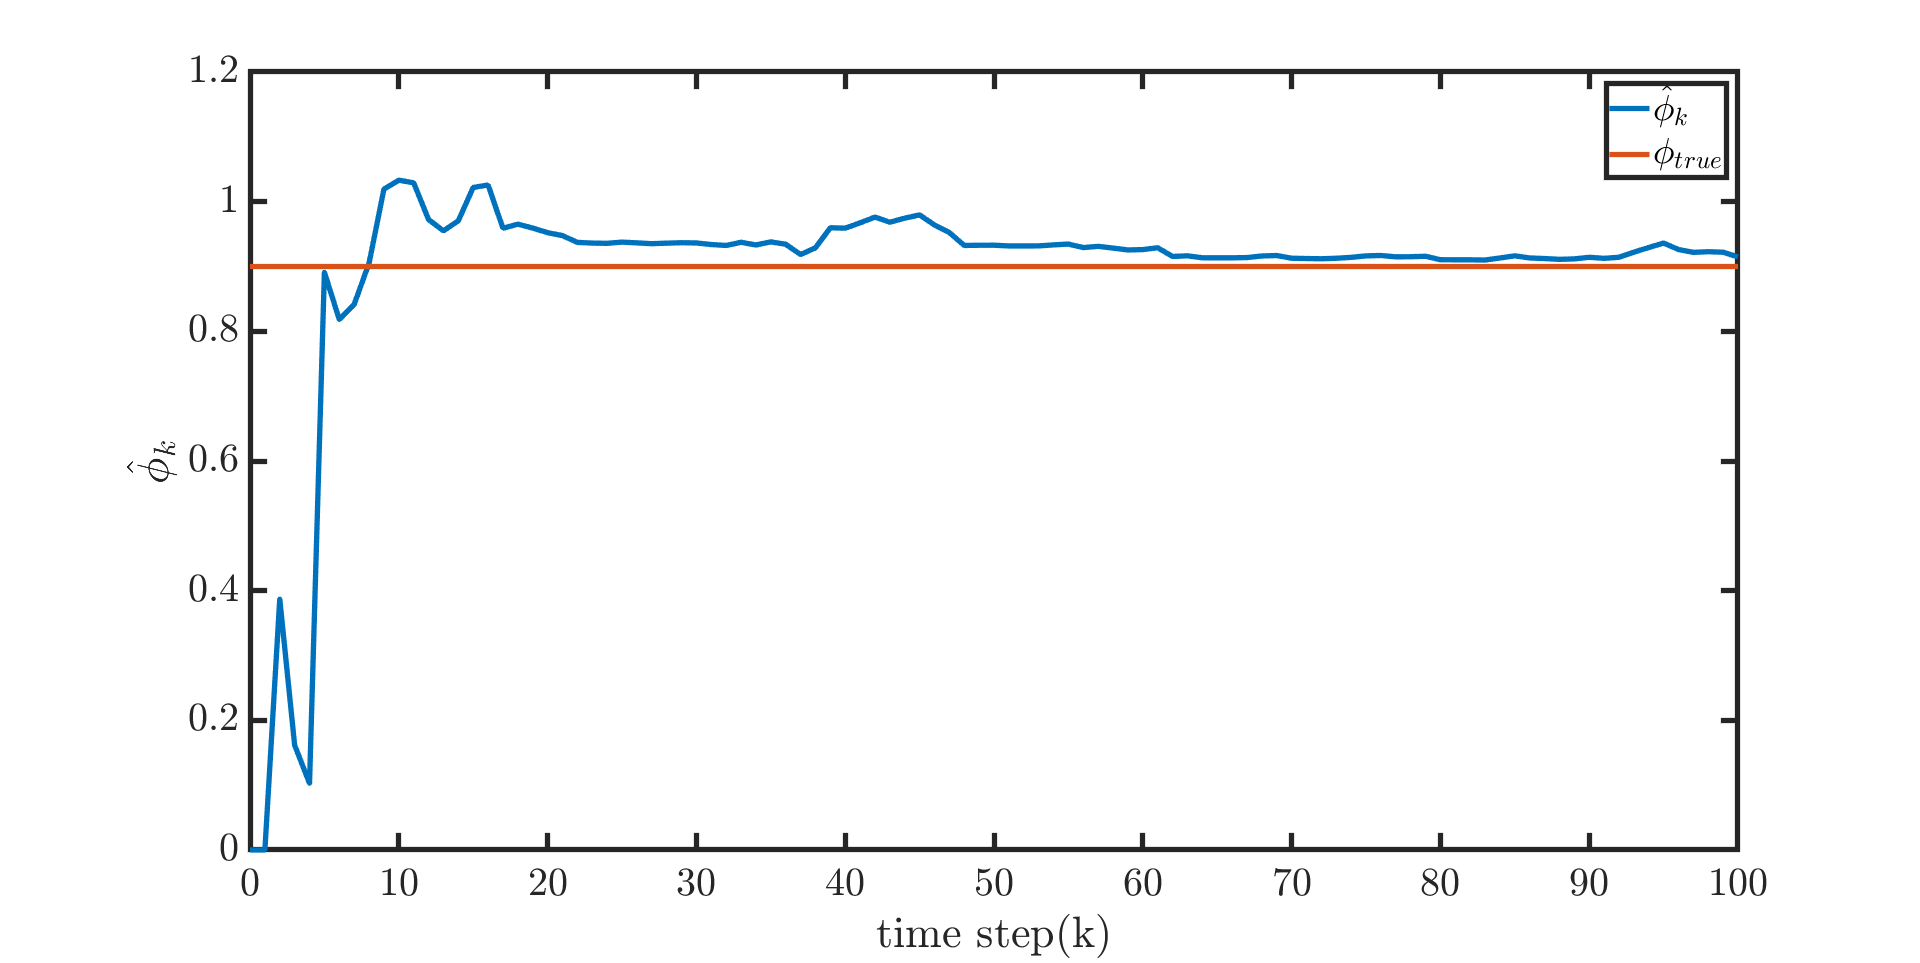
\includegraphics[scale=0.25]{q2.png}
%    \caption{Plot showing $\hat{\phi}$ as a function of time.}
%    \label{fig_q2l}
%\end{figure}
%\end{solution} 
%\lstinputlisting{HW6Q2.m}
%\noindent\rule{7in}{2.8pt}
%%%%%%%%%%%%%%%%%%%%%%%%%%%%%%%%%%%%%%%%%%%%%%%%%%%%%%%%%%%%%%%%%%%%%%%%%

%\begin{thebibliography}{1}
%\bibitem{ref}
%{\sc Author.}
%\newblock Title.
%\newblock In {\em Proc.} ..., pages xx--xx, year.
%\end{thebibliography}


\end{document}
 